\documentclass{standalone}
\usepackage{pgfplots}
\pgfplotsset{compat=1.17}

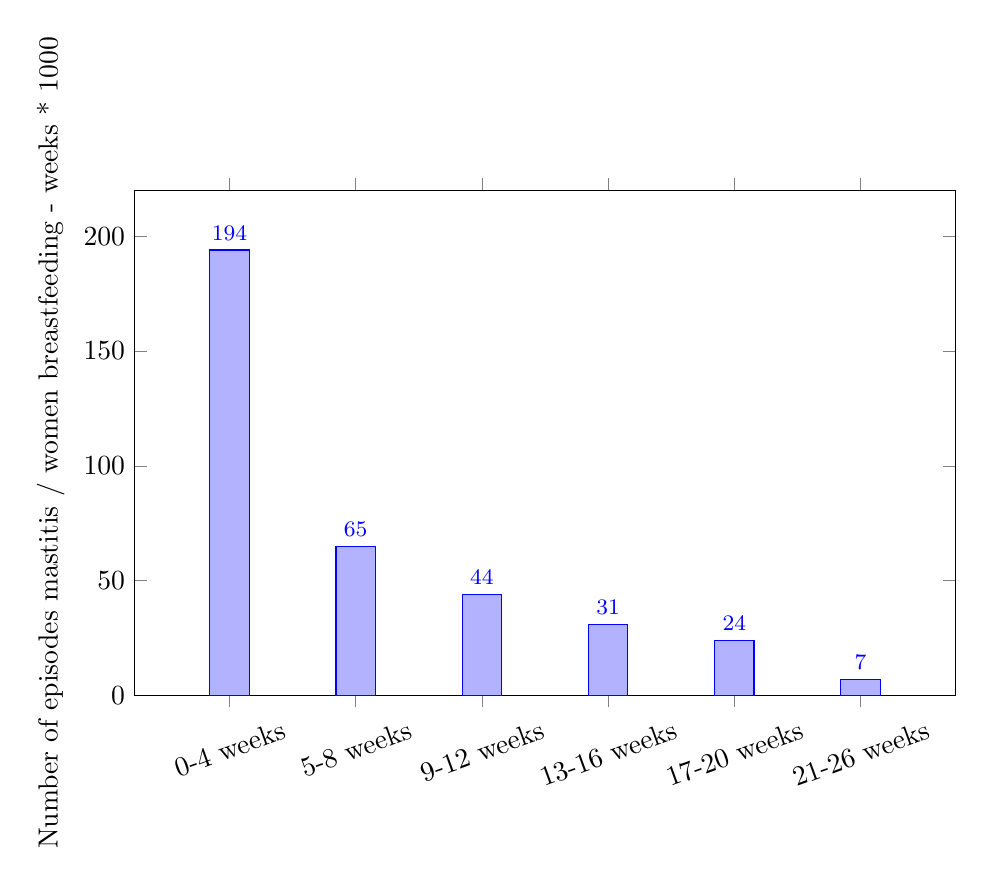
\begin{tikzpicture}
    \begin{axis}[
        ybar,
        bar width=0.5cm,
        width=12cm,
        height=8cm,
        enlarge x limits=0.15,
        ymin=0, ymax=220,
        ylabel={Number of episodes mastitis / women breastfeeding - weeks * 1000},
        symbolic x coords={0-4 weeks, 5-8 weeks, 9-12 weeks, 13-16 weeks, 17-20 weeks, 21-26 weeks},
        xtick=data,
        nodes near coords,
        every node near coord/.append style={font=\footnotesize, anchor=south},
        nodes near coords align={vertical},
        x tick label style={rotate=20}
    ]
        \addplot coordinates {(0-4 weeks,194) (5-8 weeks,65) (9-12 weeks,44) (13-16 weeks,31) (17-20 weeks,24) (21-26 weeks,7)};
    \end{axis}
\end{tikzpicture}
\end{document}